\documentclass{book}
\usepackage[paperwidth=36in,paperheight=60in,hmargin=0.75in,vmargin=0.75in]{geometry}
\usepackage{graphicx}
\usepackage{ae}

\begin{document}

\setlength{\unitlength}{1in}
\begin{picture}(34.5,58.5){}
\linethickness{0.125in}

%%%%% POSTER BORDER
\put(0,0.0625){\line(1,0){34.4375}}
\put(0,58.375){\line(1,0){34.4375}}
\put(0,0){\line(0,1){58.4375}}
\put(34.375,0){\line(0,1){58.4375}}

%%%%% TITLE TYPE TEXT
\put(0,55.25){
  \makebox(34.5,2.5){
    \centering
    % title
    \fontsize{180}{200}\selectfont Mapping Chaos
  }
}
\put(0,1.5){
  \makebox(34.25,1.5){
    \centering
    % required siggraph name
    \fontsize{100}{120}\selectfont SIGGRAPH 2004
  }
}
\put(0,0.5){
  \makebox(34.25,1){
    \centering
    % required siggraph location
    \fontsize{80}{100}\selectfont Los Angeles, California
  }
}

%%%%% NAMES, CONTACT INFO
\put(0,53.75){
  \makebox(17,0.8334){
    \centering
    \fontsize{60}{70}\selectfont David Trowbridge
  }
}
\put(0,52.9333){
  \makebox(17,0.6944){
    \centering
    \fontsize{50}{60}\selectfont trowbrds@cs.colorado.edu
  }
}
\put(17.5,53.75){
  \makebox(17,0.8334){
    \centering
    \fontsize{60}{70}\selectfont Micah Dowty
  }
}
\put(17.5,52.9333){
  \makebox(17,0.6944){
    \centering
    \fontsize{50}{60}\selectfont micah@navi.cx
  }
}

\linethickness{0.0625in}

%%%%% GENERAL OVERVIEW
\put(0.75,40){
  \parbox{32.75in}{
    \fontsize{60}{70}\selectfont
    Traditional imaging techniques for visualizing systems such as chaotic
    maps are usually extremely simple, darkening pixels directly as the
    point moves around the image region with each iteration. This allows
    only a few thousand points to be drawn, resulting in a crude image.
    Instead, by treating the entire region as a two dimensional histogram,
    the function can be iterated millions or even billions of times,
    dramatically increasing the information visible to the eye. This results
    in a high dynamic range image which can then be processed and interpolated
    to enhance or explore the final result. This interpolation step is
    computationally trivial compared to the map iteration, so it can be
    performed repeatedly, allowing the user to explore parameter spaces
    interactively and then watch the image develop more and more detail.
  }
}

%%%%% IMAGE COMPARISON - HDR INTERPOLATION
%%% text
\put(0.75,14.5){
  \parbox{32.75in}{
    \centering
    \fontsize{60}{70}\selectfont
    Because the image is computed with a high dynamic range, it can be
    interpolated differently to bring out different details. Because
    this step is done separately from computing the image, it can be
    changed in real time, allowing the viewer to tweak the parameters
    to produce the desired effect.
  }
}
%%% base image
\put(0.75,5){
  
\includegraphics[width=8in]{images/base.png}
}
\put(0.75,4){
  \makebox(8,1){
    \centering
    \fontsize{50}{60}\selectfont Base Image
  }
}

%%% increased exposure
\put(8.75,5){
  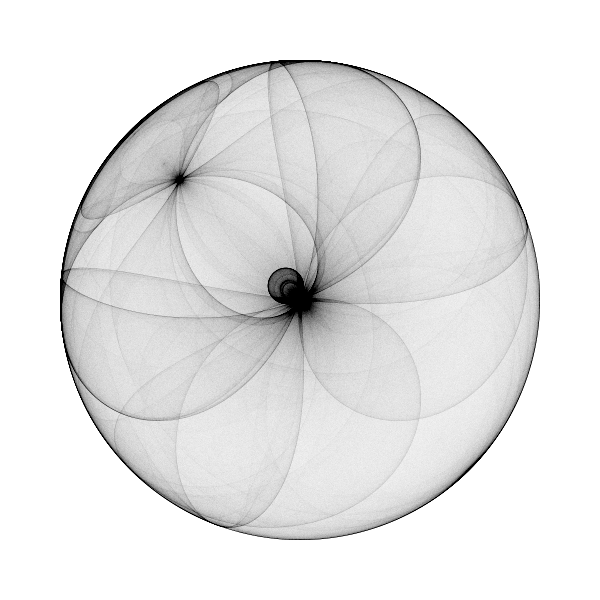
\includegraphics[width=8in]{images/increased-exposure.png}
}
\put(8.75,4){
  \makebox(8,1){
    \centering
    \fontsize{50}{60}\selectfont Increased Exposure
  }
}

%%% increased gamma
\put(17.25,5){
  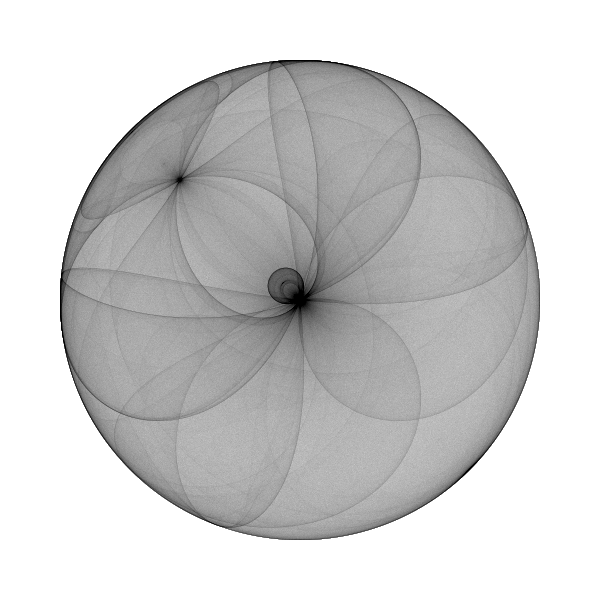
\includegraphics[width=8in]{images/increased-gamma.png}
}
\put(17.25,4){
  \makebox(8,1){
    \centering
    \fontsize{50}{60}\selectfont Increased Gamma
  }
}

%%% decreased exposure, increased gamma
\put(25.75,5){
  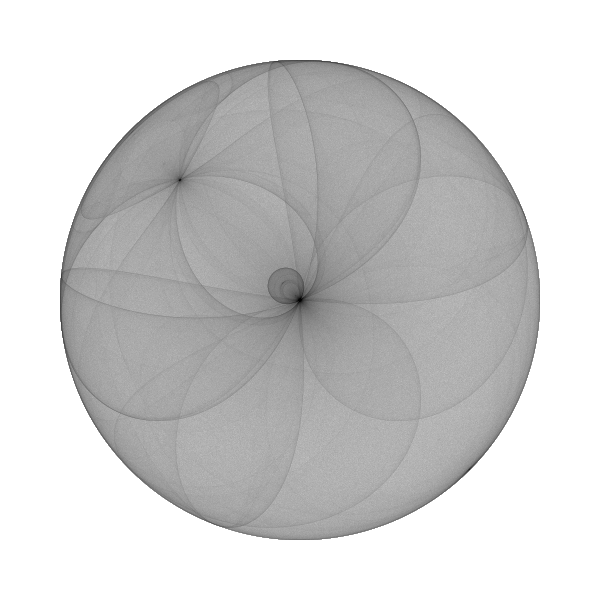
\includegraphics[width=8in]{images/decreased-exposure-increased-gamma.png}
}
\put(25.75,4.347){
  \makebox(8,1){
    \centering
    \fontsize{50}{60}\selectfont Decreased Exposure,
  }
}
\put(25.75,3.6527){
  \makebox(8,1){
    \centering
    \fontsize{50}{60}\selectfont Increased Gamma
  }
}

\end{picture}

\end{document}
